\documentclass[11pt]{article}

\usepackage{amsmath, amssymb}
\usepackage[margin=1in]{geometry}
\usepackage{hyperref}
\usepackage{graphicx}

\title{Actor-Parallel Multi-Fidelity Bayesian Optimization\\ for $\beta$-VAE Hyperparameter Tuning}
\author{}
\date{}

\begin{document}
\maketitle

\section{Maximum Mean Discrepancy as the Optimization Objective}
\label{sec:mmd}

Every candidate hyperparameter needs a single scalar score, and that score
has to capture something more demanding than reconstruction error: whether
samples \emph{generated from scratch} by the full pipeline are
statistically indistinguishable from real data. We use Maximum Mean
Discrepancy (MMD) for this, a kernel-based two-sample test statistic that
measures the distance between two distributions using only samples drawn
from each, with no need for either distribution's density to be tractable.
For distributions $P$ and $Q$ and a characteristic kernel $k$,
\begin{equation}
\mathrm{MMD}^2(P, Q) = \mathbb{E}_{x, x' \sim P}[k(x, x')]
  + \mathbb{E}_{y, y' \sim Q}[k(y, y')]
  - 2\,\mathbb{E}_{x \sim P,\, y \sim Q}[k(x, y)],
\end{equation}
which is zero if and only if $P = Q$, and otherwise grows with how
separated the two distributions are in the kernel's feature space.

In our setting, $P$ is the true data distribution, represented by a batch
of held-out real samples, and $Q$ is the distribution induced by the
trained generative pipeline: Gaussian noise is drawn in the VAE's latent
space and transported by a learned flow-matching velocity field (a
short ODE integration) into the shape of the encoder's aggregate
posterior, and the result is passed through the VAE decoder back into
data space. $\mathrm{MMD}^2$ is then estimated empirically from an equal
number of real and generated samples using an RBF kernel, with the
kernel bandwidth set once by the median heuristic over the pooled
real-and-generated pairwise distances and reused identically for all
three terms above — using a different bandwidth per term would break the
guarantee that the estimator stays non-negative. The resulting score is
floored at zero to absorb floating-point round-off and reported on a
$\log_{10}$ scale, since MMD values across the $\beta$ search range span
several orders of magnitude.

A lower MMD means the generative pipeline's samples are a
closer statistical match to real data, and it is exactly this score,
as a function of $\beta$, that the optimizer is trying to minimize.

\section{Our Method}
\label{sec:method}

\subsection{Task}
\label{sec:task}

The hyperparameter being tuned is $\beta$, the weight on the KL term of
the $\beta$-VAE's evidence lower bound,
\begin{equation}
\mathcal{L}(\beta) = \mathbb{E}_q\!\left[\log p(x \mid z)\right]
  - \beta \, D_{\mathrm{KL}}\!\left(q(z \mid x)\,\|\,p(z)\right).
\end{equation}
$\beta$ controls how strongly the encoder's aggregate posterior is pulled
toward the prior; too small and the flow-matching model has to sample
from a latent distribution with gaps and irregular structure it was never
trained to cross, too large and reconstruction quality collapses. Neither
failure mode is visible from a closed-form expression, so $\beta$ can only
be judged by the MMD score of Section~\ref{sec:mmd}, measured after
training the full VAE + flow-matching pipeline to convergence.

A good $\beta$ can lie anywhere from $10^{-8}$ to $10^{1}$, so the
optimizer never searches directly in $\beta$-space. It instead works over
a normalized coordinate $u \in [0,1]$ that maps linearly onto
$\log_{10}\beta$, with $\beta$ recovered by exponentiating; this gives a
Gaussian process surrogate a single fixed lengthscale that is meaningful
across the whole range, rather than one dominated by the nine-decade gap
between the smallest and largest candidates considered. The surrogate
itself is a GP with a squared-exponential (RBF) kernel,
\begin{equation}
k(u, u') = \exp\!\left(-\frac{(u-u')^2}{2\ell^2}\right),
\end{equation}
fit over $\log_{10}(\mathrm{MMD})$ as a function of $u$, with a small
diagonal nugget added both for numerical stability and to reflect that a
training run is a noisy measurement rather than an exact one.

Because a full training run is expensive (on the order of tens of minutes
per candidate), every candidate $u$ can be scored in two different ways
that are not equally costly:
\begin{itemize}
  \item a \textbf{GP run} — the surrogate's own posterior mean and
    standard deviation at $u$, computed from whatever real observations
    it has seen so far. This is free: nothing is trained, and the result
    is never treated as ground truth, only as an estimate of what a real
    run at $u$ would likely return.
  \item a \textbf{full run} — the actual VAE + flow-matching pipeline
    trained end to end at $u$, with the resulting MMD fed back into the
    surrogate as a genuine observation.
\end{itemize}
The task, then, is to decide — from the free, whole-search-space picture
a GP run gives at no cost — which small number of candidates are worth
spending a real full run on, and to do so while making use of parallel
hardware rather than one run at a time.

\subsection{Setting up Actors}
\label{sec:actors}

A full run's cost is entirely wall-clock time spent training, which
parallelizes cleanly across independent candidates. We exploit this with
a manager–worker actor pattern built on the C++ Actor Framework (CAF):

\begin{itemize}
  \item A single \textbf{manager actor} owns the optimization state (the
    GP surrogate and its observation history) and drives the loop one
    round at a time: it proposes a batch of candidate $u$ values
    (Section~\ref{sec:sampling}), dispatches one job per candidate, waits
    for every job in the round to report back, folds each result into the
    surrogate, and only then proposes the next batch.
  \item For every job in a round, an ephemeral \textbf{worker actor} is
    spawned whose sole responsibility is that one candidate. Each worker
    launches its full training run as an independent subprocess and,
    once it exits, sends the resulting MMD back to the manager as an
    asynchronous message before shutting down.
\end{itemize}

Because actors communicate only through asynchronous messages and never
share mutable state directly, the manager's mailbox naturally serializes
result handling — results can arrive in any order, from any number of
concurrently running workers, without explicit locks — while each worker
actor is free to block on its own long training run without stalling
anything else in the system.

Within a round, every worker actor in that round's batch runs
concurrently; the manager blocks only until all of them have reported
back, then tears the round down before proposing the next batch. This
makes parallelism strictly \emph{within} a round while rounds themselves
stay sequential, which matches the requirement that the surrogate must
see a full round's results before the next batch can be chosen
meaningfully. Available GPUs are treated as a shared pool and assigned to
workers round-robin — as each worker actor is dispatched it claims the
next GPU in rotation — so a round's concurrent training jobs spread
evenly across all available hardware instead of contending for one
device. Both the number of parallel workers and the number of GPUs to
round-robin across are configurable, letting the same loop scale from a
single GPU up to several.

\subsection{Smart Sampling}
\label{sec:sampling}

At each round, the surrogate's posterior mean $\mu$ and standard
deviation $\sigma$ are evaluated on a dense, evenly spaced grid over
$u \in [0,1]$, and every grid point is scored by
\begin{equation}
a(u) = y_{\text{best}} - \mu(u) + \sigma(u),
\end{equation}
where $y_{\text{best}}$ is the best (lowest) $\log_{10}(\mathrm{MMD})$
observed so far. The first two terms favor points the surrogate predicts
will beat the current best (exploitation); the $\sigma(u)$ term favors
points the model is still unsure about (exploration). This is the same
exploitation/exploration balance canonical acquisition functions such as
expected improvement or upper confidence bound are designed to strike,
here expressed as a simple additive score.

A single best-scoring point is not useful when a whole batch of workers
is available to fill at once: naively taking the top-$k$ grid points
would cluster them all around the same peak of $a(u)$, wasting parallel
workers on near-duplicate evaluations. Instead, candidates are ranked by
$a(u)$ and accepted greedily subject to a minimum separation constraint —
a candidate is only added to the batch if it lies at least a fixed
minimum distance away, in normalized $u$-space, from every point already
in the batch \emph{and} from every point evaluated in any previous round.
This spreads a round's evaluations across distinct regions of interest
and, just as importantly, stops the optimizer from re-running a $\beta$
it has already measured. If the search space is saturated enough that
fewer than the required number of well-separated candidates remain, the
separation constraint against \emph{history} is relaxed just enough to
fill out the batch, so every round still produces a full batch of work
while preferring unexplored candidates whenever they exist. Since a GP
run costs nothing and is never itself scheduled as a job, every candidate
that survives this selection is evaluated the same way: as a full run.

\section{Experiment and Results}
\label{sec:experiments}

Three drivers implement the task of Section~\ref{sec:task} and are
compared against each other throughout this section. All three run the
identical schedule — a 3-point seed followed by 10 acquisition rounds of
3 candidates each, 33 real \texttt{latentflow1.py} full runs in total —
over the identical $\log_{10}\beta$ search space, so any difference
between them is attributable to the one thing each pair changes, not to
the task itself:
\begin{itemize}
  \item \textbf{\texttt{mfbo\_demo} — sequential baseline.} Our own GP
    and acquisition logic (Section~\ref{sec:method}), no actors: each
    round's batch of candidates is evaluated one full run at a time, in a
    single process.
  \item \textbf{\texttt{mfbo\_hf} — actor-parallel.} The identical GP and
    acquisition logic as \texttt{mfbo\_demo}, but each round's batch is
    dispatched to independent worker actors that train concurrently,
    round-robined across the machine's GPUs (Section~\ref{sec:actors}).
  \item \textbf{\texttt{mfbo\_botorch} — library baseline.} The same
    parallel, round-robined dispatch as \texttt{mfbo\_hf}, but with the
    GP surrogate and acquisition logic replaced by BoTorch's, detailed in
    Table~\ref{tab:botorch-mapping}.
\end{itemize}
\texttt{mfbo\_demo} vs.\ \texttt{mfbo\_hf} isolates the wall-clock benefit
of evaluating a batch concurrently rather than sequentially, holding the
GP/acquisition logic fixed (Section~\ref{sec:parallelism-result}).
\texttt{mfbo\_hf} vs.\ \texttt{mfbo\_botorch} isolates what our
hand-rolled surrogate and acquisition logic costs or gains relative to a
mature library implementation, holding parallelism fixed
(Section~\ref{sec:library-result}). All three schedule only full runs —
the GP-run tier is queried purely for the free prediction curve, never as
a substitute evaluation.

\subsection{Validation Methodology}
\label{sec:validation}

Two checks back the numbers in this section. First, a component-level
substitution: \texttt{mfbo\_botorch.py} targets the exact same task as
\texttt{mfbo\_hf} — same search space, same seed/round/batch schedule,
same real evaluations, same GPU dispatch — with every piece of custom
numerical code swapped for its BoTorch library equivalent, summarized in
Table~\ref{tab:botorch-mapping}. Holding everything else fixed makes the
comparison in Section~\ref{sec:library-result} a fair one.

\begin{table}[htbp]
\centering
\begin{tabular}{p{3.1cm}p{5.3cm}p{5.3cm}}
\hline
\textbf{Component} & \textbf{\texttt{mfbo\_hf} (this work)} & \textbf{\texttt{mfbo\_botorch} (baseline)} \\
\hline
GP surrogate &
  hand-written RBF kernel and Cholesky solve, fixed lengthscale &
  \texttt{SingleTaskGP} (GPyTorch), lengthscale and noise fit by
  marginal-likelihood optimization \\[4pt]
Acquisition &
  $a(u) = y_{\text{best}} - \mu(u) + \sigma(u)$, an ad hoc
  exploit/explore score &
  \texttt{qLogExpectedImprovement} (used for the run reported here); \texttt{qKnowledgeGradient} also available via \texttt{--acquisition kg} \\[4pt]
Batch diversity &
  greedy candidate selection under a hand-tuned minimum-separation
  rule &
  joint optimization of the $q$ candidates against their joint
  posterior (\texttt{optimize\_acqf}) \\[4pt]
Parallel dispatch &
  CAF manager/worker actors, one \texttt{std::thread} per job &
  a Python thread pool, one thread per job \\[4pt]
GPU assignment &
  round-robin \texttt{CUDA\_VISIBLE\_DEVICES} &
  identical round-robin \texttt{CUDA\_VISIBLE\_DEVICES} \\
\hline
\end{tabular}
\caption{Component-by-component mapping between the custom
\texttt{mfbo\_hf} driver and the BoTorch baseline \texttt{mfbo\_botorch}.}
\label{tab:botorch-mapping}
\end{table}

Second, a methodology-level sanity check, still open: comparing our
sequential optimization loop against BoTorch run with a Knowledge
Gradient acquisition function on standard synthetic benchmark functions
with \emph{known} global optima. Knowledge Gradient is a one-step-lookahead
rule — it explicitly estimates the expected improvement to the posterior
mean at the incumbent optimum from evaluating a candidate, a more
principled (if more expensive) baseline than
Section~\ref{sec:sampling}'s ad hoc score. Because the real MMD objective
has no known optimum to check against, this benchmark comparison is what
would confirm whether any gap seen in Section~\ref{sec:library-result} is
a genuine modeling limitation rather than an artifact of a single 33-run
trial per driver. \emph{This synthetic-benchmark run has not been done
yet — see Section~\ref{sec:takeaways}.}

\subsection{Wall-Clock Time}
\label{sec:parallelism-result}

\begin{table}[htbp]
\centering
\begin{tabular}{lccc}
\hline
\textbf{Driver} & \textbf{Full runs} & \textbf{Wall time} & \textbf{Speedup vs.\ \texttt{mfbo\_demo}} \\
\hline
\texttt{mfbo\_demo} (sequential) & 33 & $\approx$39 min & $1.0\times$ (baseline) \\
\texttt{mfbo\_hf} (actor-parallel) & 33 & $\approx$14 min & $\approx$2.8$\times$ \\
\texttt{mfbo\_botorch} (library, parallel) & 33 & $\approx$16 min & $\approx$2.5$\times$ \\
\hline
\end{tabular}
\caption{Wall-clock time for all 33 full runs, each driver's own timed
run.}
\label{tab:wallclock}
\end{table}

\texttt{mfbo\_hf} and \texttt{mfbo\_botorch} both dispatch a round's
batch of three candidates concurrently, round-robined across two GPUs, so
both finish in roughly a third of \texttt{mfbo\_demo}'s sequential time.
\texttt{mfbo\_botorch} runs about two minutes slower than \texttt{mfbo\_hf}
over the 11 rounds — GP-fitting via marginal-likelihood optimization and
joint batch-acquisition optimization (\texttt{optimize\_acqf}) are
themselves more expensive per round than our fixed-lengthscale GP and
closed-form score, but that overhead (tens of seconds per round) is small
next to a full training run (multiple minutes), so it barely erodes the
parallelism benefit.

\subsection{Solution Quality}
\label{sec:library-result}

\begin{table}[htbp]
\centering
\begin{tabular}{lccc}
\hline
\textbf{Driver} & \textbf{Best $\beta$} & \textbf{Best MMD} & \textbf{Relative to best} \\
\hline
\texttt{mfbo\_demo} (sequential) & $0.0115$ & $3.56\times 10^{-3}$ & $+13\%$ \\
\texttt{mfbo\_hf} (actor-parallel) & $0.0030$ & $3.58\times 10^{-3}$ & $+14\%$ \\
\texttt{mfbo\_botorch} (library, parallel) & $0.0089$ & $\mathbf{3.15\times 10^{-3}}$ & best \\
\hline
\end{tabular}
\caption{Best MMD found by each driver over its 33 full runs. "Relative
to best" is the percent by which that driver's best MMD exceeds the
lowest MMD found across all three.}
\label{tab:quality}
\end{table}

\texttt{mfbo\_demo} and \texttt{mfbo\_hf} — identical GP and acquisition
logic, differing only in parallelism — land in the same low-$\beta$ basin
and within 1\% of each other's best MMD, exactly as expected: parallelizing
a round changes only the order results arrive in, not which candidates
the acquisition step chooses. \texttt{mfbo\_botorch} finds a best MMD
roughly 12--14\% lower than either custom driver, at a different point in
the same basin ($\beta \approx 0.009$ rather than $\beta \approx
0.003$–$0.011$). Since \texttt{mfbo\_botorch} matches \texttt{mfbo\_hf}'s
parallelism (Table~\ref{tab:wallclock}), this gap is attributable to the
surrogate/acquisition side of Table~\ref{tab:botorch-mapping} — most
plausibly the marginal-likelihood-fit lengthscale (vs.\ our fixed
$\ell=0.1$) and the closed-form \texttt{qLogExpectedImprovement} score
(vs.\ our ad hoc $a(u)$) — rather than to how much of the search budget
each driver could run concurrently.

\subsection{Result Curves}

Figures~\ref{fig:mfbo-demo}, \ref{fig:mfbo-hf}, and~\ref{fig:mfbo-botorch}
plot, for each driver, the GP's low-fidelity prediction curve (mean
$\pm\,1\sigma$, in blue) over the full $\beta$ range against every full
run actually performed (points, colored by the order in which that run
completed, with the best result starred). Under \texttt{mfbo\_demo}, run
order tracks proposal order exactly. Under \texttt{mfbo\_hf} and
\texttt{mfbo\_botorch}, several full runs are in flight at once, so
completion order can differ from proposal order.

\begin{figure}[htbp]
  \centering
  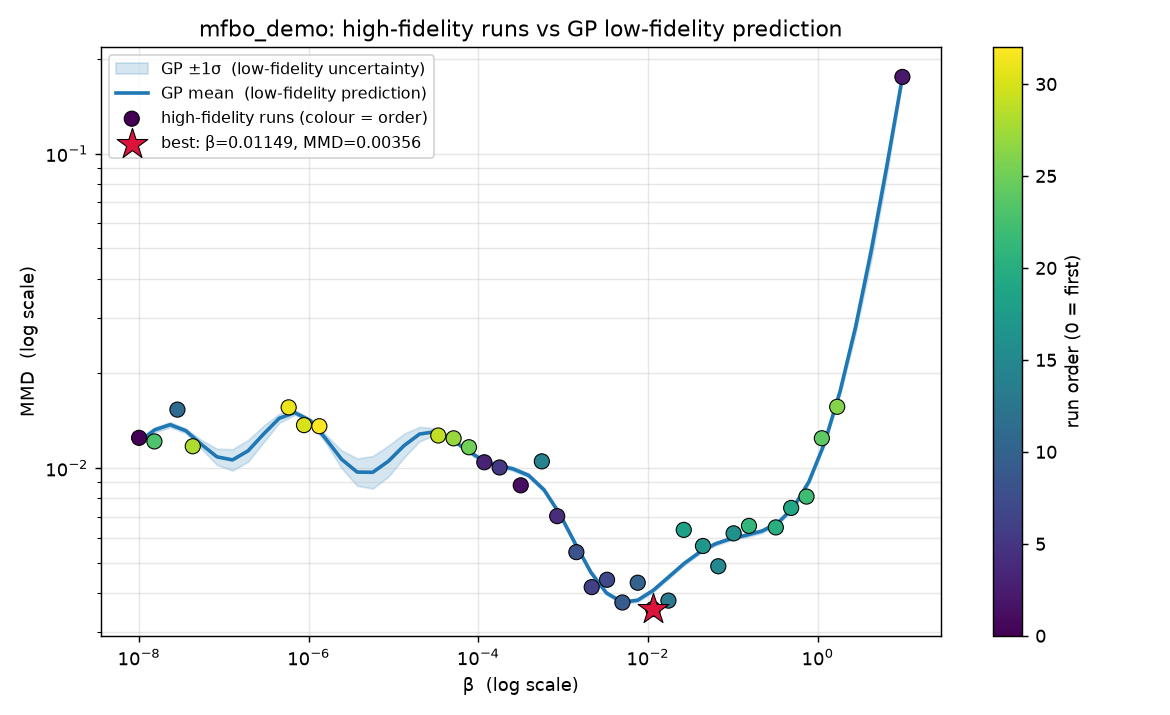
\includegraphics[width=0.85\textwidth]{figs/mfbo_demo.png}
  \caption{Sequential baseline (\texttt{mfbo\_demo}, no actors): GP
    low-fidelity prediction vs.\ full runs.}
  \label{fig:mfbo-demo}
\end{figure}

\begin{figure}[htbp]
  \centering
  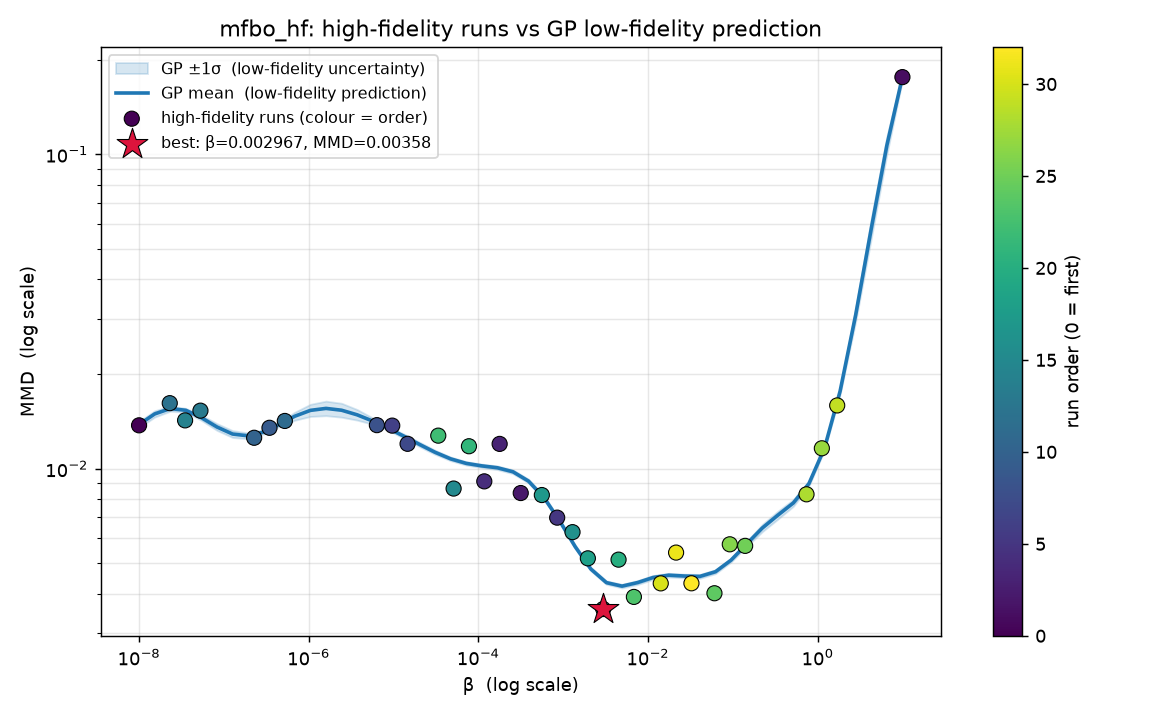
\includegraphics[width=0.85\textwidth]{figs/mfbo_hf.png}
  \caption{Actor-parallel driver (\texttt{mfbo\_hf}): GP low-fidelity
    prediction vs.\ full runs, dispatched concurrently across worker
    actors.}
  \label{fig:mfbo-hf}
\end{figure}

\begin{figure}[htbp]
  \centering
  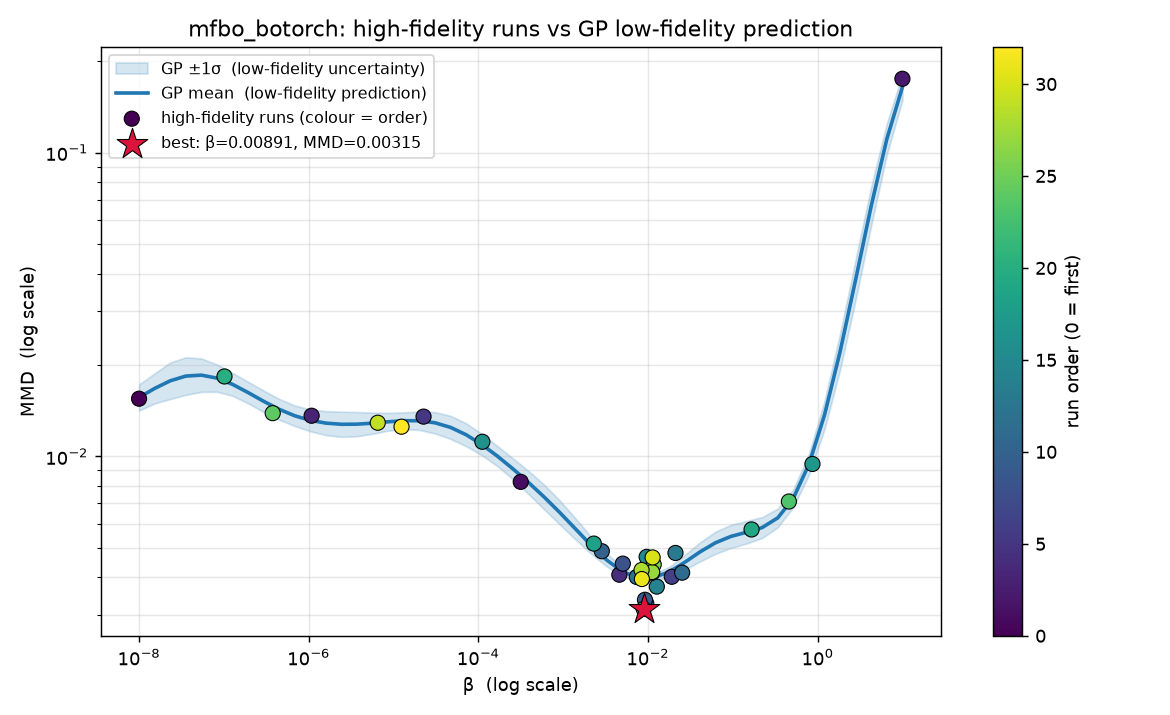
\includegraphics[width=0.85\textwidth]{figs/mfbo_botorch.png}
  \caption{BoTorch library baseline (\texttt{mfbo\_botorch}): GP
    low-fidelity prediction vs.\ full runs, dispatched with the same
    round-robin GPU parallelism as \texttt{mfbo\_hf}.}
  \label{fig:mfbo-botorch}
\end{figure}

\subsection{Key Takeaways for Continuation}
\label{sec:takeaways}

\begin{itemize}
  \item \textbf{The actor layer is already close to library-parallel
    cost.} \texttt{mfbo\_hf} and \texttt{mfbo\_botorch} finish within
    about two minutes of each other (Table~\ref{tab:wallclock}), so the
    custom CAF actor layer is not leaving significant wall-clock
    performance on the table relative to a Python thread pool doing the
    same round-robined dispatch.
  \item \textbf{The GP/acquisition side is where the gap is.} BoTorch's
    library GP and \texttt{qLogExpectedImprovement} found a best MMD
    12--14\% lower than either custom driver
    (Table~\ref{tab:quality}) for essentially the same wall-clock cost as
    \texttt{mfbo\_hf}. The highest-value next step for this project is
    almost certainly upgrading \texttt{mfbo.h}'s GP/acquisition —
    fitting the RBF lengthscale and noise by marginal likelihood instead
    of the fixed $\ell = 0.1$, and/or replacing the ad hoc score
    $a(u) = y_{\text{best}} - \mu(u) + \sigma(u)$ with a real expected-improvement
    calculation — rather than further optimizing the actor/parallelism
    layer.
  \item \textbf{Open validation work.} The synthetic-benchmark check
    against BoTorch + Knowledge Gradient described in
    Section~\ref{sec:validation} has not been run. It would confirm
    whether the quality gap above is a genuine modeling limitation of the
    hand-rolled GP/acquisition or noise from comparing single 33-run
    trials.
  \item \textbf{Where everything lives.} All three drivers'
    (\texttt{mfbo\_demo}, \texttt{mfbo\_hf}, \texttt{mfbo\_botorch}) raw
    run data is in \texttt{actors/} as matching
    \texttt{*\_runs.csv}/\texttt{*\_pred.csv} pairs; \texttt{plot\_mfbo.py}
    regenerates the comparison figure from any pair, so a re-run of any
    driver reproduces Figures~\ref{fig:mfbo-demo}--\ref{fig:mfbo-botorch}
    automatically.
\end{itemize}

\section{Summary}

The method combines three ingredients: a \textbf{free surrogate-prediction
tier} (Section~\ref{sec:task}) that lets the GP's own posterior stand in,
at zero cost, for every candidate not yet worth a real run; a
\textbf{diversity-constrained batch acquisition} strategy
(Section~\ref{sec:sampling}) that turns that free, whole-search-space
belief into a spread-out set of non-redundant candidates worth a real run
each round; and an \textbf{actor-based parallel execution layer}
(Section~\ref{sec:actors}) that evaluates an entire round's batch of full
runs concurrently across available GPUs. Measured on the real objective
(Section~\ref{sec:experiments}), the actor-parallel driver reaches the
same solution quality as the equivalent sequential driver in roughly a
third of the wall-clock time (Table~\ref{tab:wallclock}), and a BoTorch
library implementation of the same parallel driver finds a best MMD
12--14\% lower still (Table~\ref{tab:quality}) at comparable wall-clock
cost — pointing at the GP/acquisition implementation, not the actor
layer, as the highest-value target for further work
(Section~\ref{sec:takeaways}).

\end{document}
